\documentclass[11pt]{article}

\usepackage[margin=1in]{geometry}
\usepackage{graphicx}
\usepackage{float}
\usepackage{amsmath}
\usepackage{amssymb}
\usepackage{booktabs}
\usepackage[hidelinks]{hyperref}
\usepackage{xcolor}
\usepackage{enumitem}

\setlength{\parindent}{0pt}
\setlength{\parskip}{0.75em}
\setlist[itemize]{leftmargin=1.4em}

\title{\textbf{InfraDrone Engine Pipeline}}
\author{Luke Pitstick}
\date{\today}

\begin{document}

\maketitle

\section{Overview}

InfraDrone is an image-processing and machine-learning pipeline for finding road damage from drone or camera imagery. The engine starts with a raw frame, cleans it up for model inference, detects candidate damage regions, segments the exact crack or pothole shape, and then converts those model outputs into structured damage records.

The important part is that the engine does not stop at ``there is a crack somewhere in this box.'' The detection model gives the rough location, but the segmentation and post-processing stages are what make the result useful. Those stages estimate the crack geometry, split and merge branches, classify the crack subtype, and calculate measurements like length, thickness, and area.

\section{Pipeline}

At a high level, the pipeline is:

\begin{center}
\begin{tabular}{cl}
\toprule
\textbf{Step} & \textbf{Purpose} \\
\midrule
1 & Load a frame from the input queue or image source. \\
2 & Preprocess the image for road-surface contrast and model input size. \\
3 & Run YOLO detection to find cracks and potholes as bounding boxes. \\
4 & Crop each detected region so segmentation only sees the relevant area. \\
5 & Run YOLO segmentation to create binary masks for each damage region. \\
6 & Skeletonize the masks and analyze crack branches. \\
7 & Merge branch fragments that are close and directionally aligned. \\
8 & Measure dimensions and classify the damage subtype. \\
9 & Return a structured \texttt{Damage} record for downstream reporting. \\
\bottomrule
\end{tabular}
\end{center}

In code, the top-level \texttt{Engine} wires together \texttt{DetectionEngine} and \texttt{SegmentationEngine}. The current implementation is:

\[
I \rightarrow I' \rightarrow D \rightarrow \{C_i\} \rightarrow \{M_i\}
\rightarrow \{S_i\} \rightarrow \{B_i\} \rightarrow \texttt{Damage}
\]

where \(I\) is the original image, \(I'\) is the preprocessed image, \(D\) is the detection output, \(C_i\) are cropped damage regions, \(M_i\) are segmentation masks, \(S_i\) are skeletonized masks, and \(B_i\) are final crack branches.

\section{Preprocessing}

The preprocessing step is meant to make road texture easier for the models to read. A raw frame can have glare, shadows, compression noise, and inconsistent resolution, so each image is normalized before inference.

The current preprocessing function does three things:

\begin{itemize}
    \item resizes the image to the model input size;
    \item applies CLAHE in LAB color space to improve local contrast;
    \item applies bilateral filtering to denoise while preserving edges.
\end{itemize}

Mathematically, I think of it as:

\[
I' = \operatorname{Denoise}(\operatorname{CLAHE}(\operatorname{Resize}(I))).
\]

This is a practical step more than a fancy one. Cracks are thin, low-contrast structures, so increasing local contrast before detection and segmentation helps the model see the features I care about.

\section{Detection}

The detection stage uses a YOLO model trained to find two high-level classes:

\begin{center}
\begin{tabular}{cl}
\toprule
\textbf{Class ID} & \textbf{Label} \\
\midrule
0 & Crack \\
1 & Pothole \\
\bottomrule
\end{tabular}
\end{center}

For a preprocessed image \(I'\), the detector returns bounding boxes:

\[
D = \{(x_1, y_1, x_2, y_2, c, t)\},
\]

where \(c\) is confidence and \(t\) is the predicted damage type. Detections below the configured confidence threshold are removed. The remaining boxes are cropped from the image and sent into segmentation.

This two-model design keeps the segmentation problem smaller. Instead of asking the segmentation model to understand the whole drone image, the detector narrows the input down to likely damage regions first.

\begin{figure}[H]
    \centering
    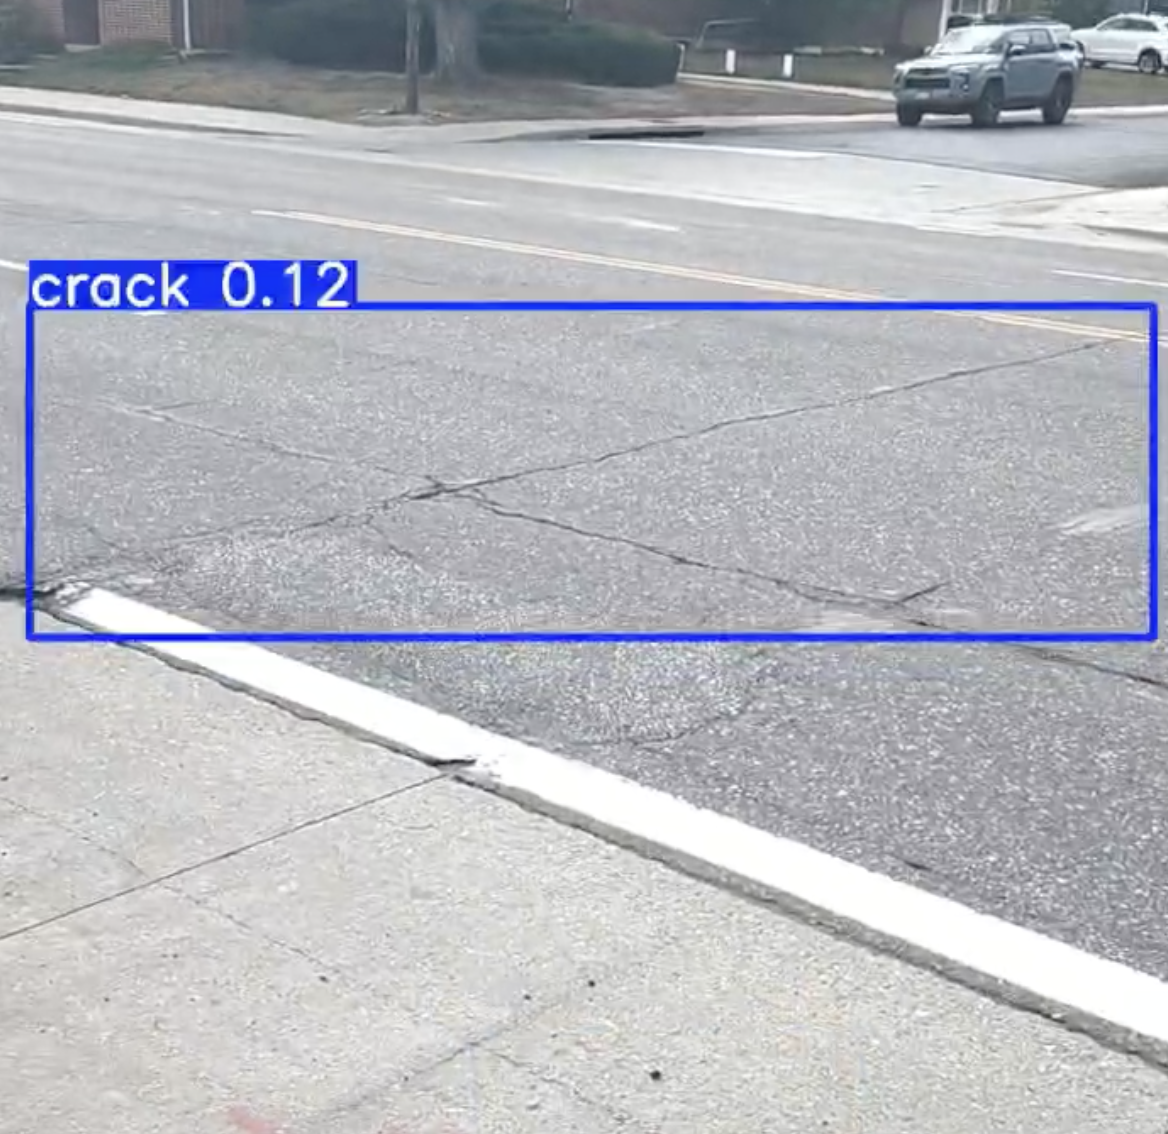
\includegraphics[width=0.82\linewidth]{screenshots/detection_crack_box.png}
    \caption{Detection output for a road crack. The blue box is the detector's crop proposal, and the class label plus confidence score are the metadata carried into the next stage.}
    \label{fig:detection-crack-box}
\end{figure}

\section{Segmentation}

The segmentation model returns a binary mask for each detected damage crop. Each mask is thresholded and skeletonized:

\[
M = \mathbf{1}(P > 0.5),
\qquad
S = \operatorname{Skeletonize}(M).
\]

The mask \(M\) keeps the full damaged area, while the skeleton \(S\) reduces the crack to a one-pixel-wide centerline. That centerline is much easier to reason about because crack length, direction, endpoints, and branches become graph-like properties instead of blob properties.

\begin{figure}[H]
    \centering
    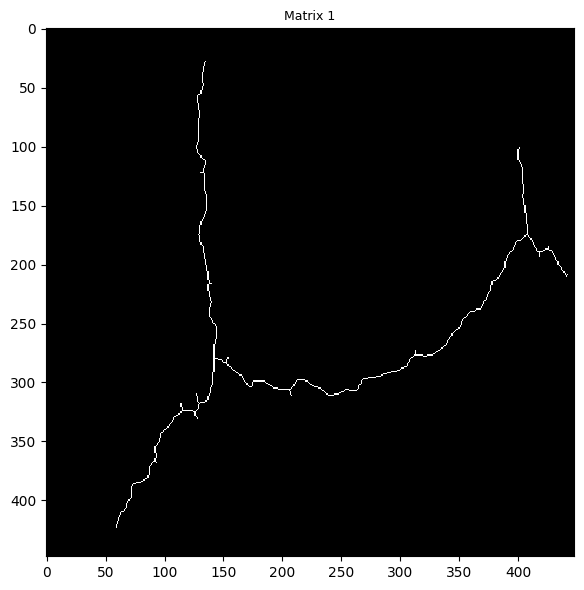
\includegraphics[width=0.72\linewidth]{screenshots/skeletonized.png}
    \caption{Skeletonized crack mask. The full segmentation mask is reduced to a one-pixel-wide centerline while preserving the shape of the crack.}
    \label{fig:skeletonized}
\end{figure}

\section{Branch Detection}

Once the crack is skeletonized, the engine searches for branch points and endpoints. A branch point is a skeleton pixel with at least three neighboring skeleton pixels in its 8-connected neighborhood:

\[
N(p) = \sum_{q \in \mathcal{N}_8(p)} S(q),
\qquad
p \text{ is a branch point if } S(p)=1 \text{ and } N(p) \geq 3.
\]

The engine dilates the branch-point region, removes it from the skeleton, and then labels the remaining connected components. Each component becomes a candidate branch. Very short components are removed so tiny artifacts do not become reported cracks.

\begin{figure}[H]
    \centering
    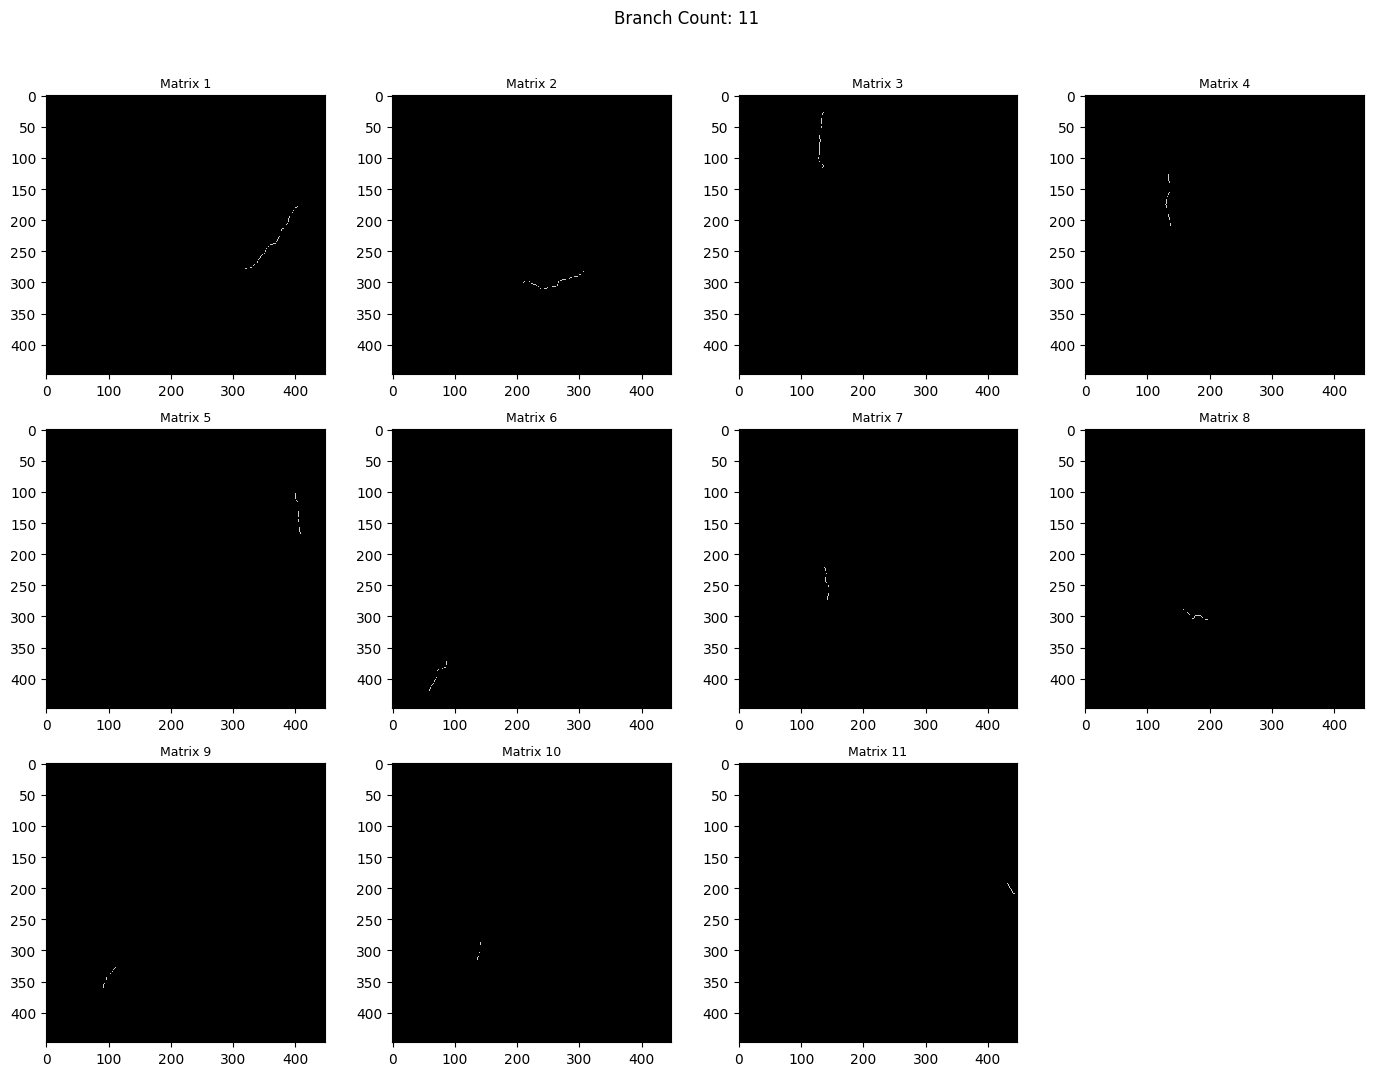
\includegraphics[width=0.9\linewidth]{screenshots/skeletonized_branches.png}
    \caption{Skeleton split into branch segments. Junction pixels are removed so connected-component labeling can isolate each branch.}
    \label{fig:split-branches}
\end{figure}

\begin{figure}[H]
    \centering
    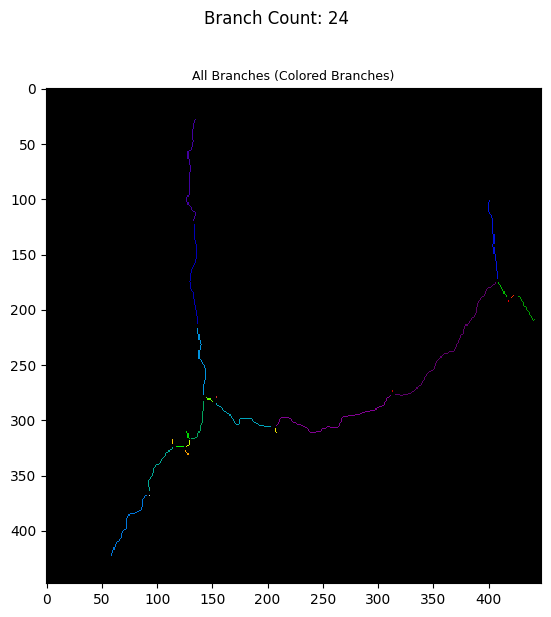
\includegraphics[width=0.7\linewidth]{screenshots/output.png}
    \caption{Colored branch labels after pruning. Each surviving component is treated as a separate branch candidate.}
    \label{fig:colored-branches}
\end{figure}

\section{Branch Angles and Merging}

Cracks often get split into multiple pieces because segmentation masks are imperfect. The engine tries to reconnect branch fragments when they are close together and point in roughly the same direction.

For each branch, the overall axis angle is estimated from the farthest pair of endpoints:

\[
\theta = \operatorname{atan2}(r_2-r_1,\ c_2-c_1) \bmod 180^\circ.
\]

The angle is treated as undirected, so \(0^\circ\) and \(180^\circ\) are equivalent. For local merge checks, the engine also estimates endpoint direction with PCA over nearby skeleton pixels. This gives a better tangent estimate at the endpoint than using the whole branch.

\begin{figure}[H]
    \centering
    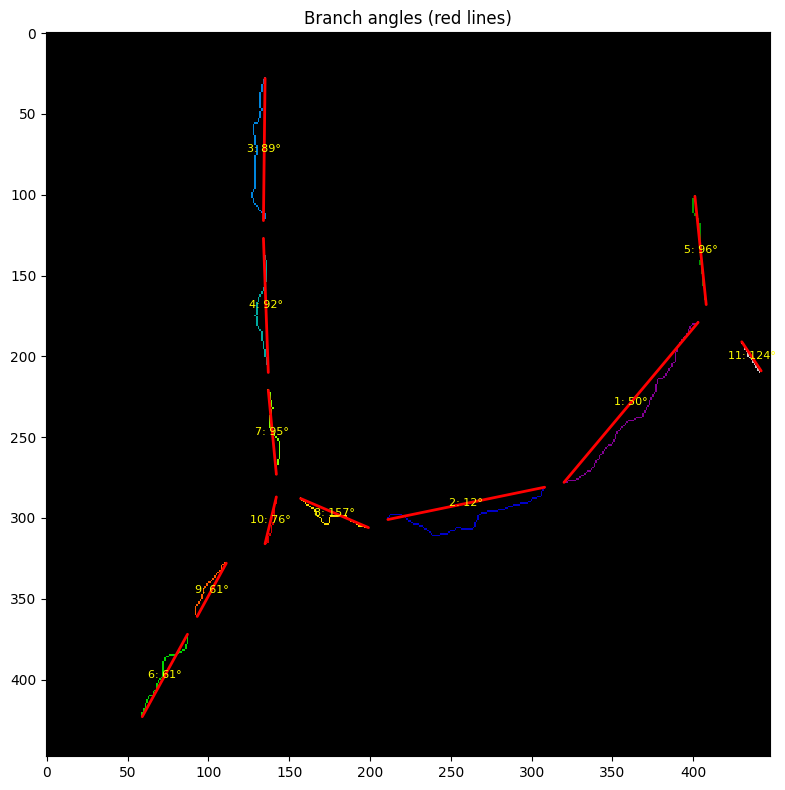
\includegraphics[width=0.72\linewidth]{screenshots/anglecalcs.png}
    \caption{Estimated branch axes. The red guide lines show the direction used for classification and merge checks.}
    \label{fig:angle-calcs}
\end{figure}

Two branches can merge if their closest endpoint distance and local angle difference are below the configured thresholds:

\[
d(e_i,e_j) < \tau_d,
\qquad
\Delta\theta(\theta_i,\theta_j) < \tau_\theta.
\]

When more than one pair is eligible, the engine chooses the lowest score:

\[
\operatorname{score} = d(e_i,e_j) + \Delta\theta(\theta_i,\theta_j).
\]

The selected pair is merged by drawing a bridge between the closest endpoints, recomputing the skeleton, and repeating until no more pairs qualify.

\begin{figure}[H]
    \centering
    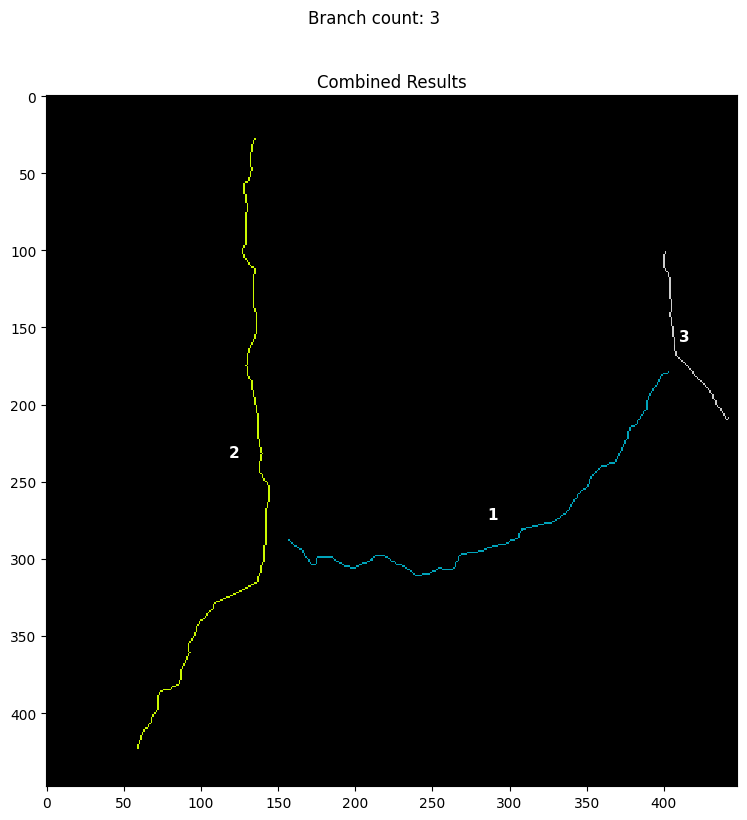
\includegraphics[width=0.72\linewidth]{screenshots/branchescomplete.png}
    \caption{Final branch groups after merging. The numbered branches are the geometry that gets passed into measurement and subtype classification.}
    \label{fig:branches-complete}
\end{figure}

\section{Measurements}

The final branch mask and skeleton are converted into physical measurements. Right now the engine stores these in pixel units unless a real-world scale ratio is configured.

\subsection{Thickness}

Thickness is estimated with a distance transform. For each skeleton pixel, the distance transform gives the distance to the nearest mask boundary. Doubling that value gives a local width estimate:

\[
w = \frac{1}{|S|}\sum_{p \in S} 2\,\operatorname{dist}(p,\partial M).
\]

This gives an average crack width across the skeleton.

\subsection{Length}

Length is currently estimated as the Euclidean distance between the farthest endpoint pair:

\[
L = \max_{e_i,e_j \in E}\|e_i-e_j\|_2.
\]

This works well for mostly straight branches. A future improvement would be to measure length along the skeleton path itself, especially for curved cracks.

\subsection{Area}

Area is the number of foreground pixels in the mask:

\[
A = \sum_{p} M(p).
\]

If the engine has a pixel-to-real-world conversion ratio, thickness, length, and area can be scaled into centimeters or inches.

\section{Subtype Classification}

After the geometry is measured, the engine assigns a crack subtype. The current rule is simple:

\begin{itemize}
    \item if the branch network has many connections, classify it as alligator cracking;
    \item otherwise classify by orientation angle;
    \item branches above the angle threshold are longitudinal;
    \item branches below the angle threshold are transverse.
\end{itemize}

This is intentionally explainable. It is not trying to hide the decision in another model. The crack subtype comes from the skeleton shape and its orientation in the image.

\section{Output Record}

Each final result becomes a \texttt{Damage} object. The record includes:

\begin{itemize}
    \item a unique ID;
    \item the final mask and skeleton;
    \item the damage type, either crack or pothole;
    \item confidence;
    \item thickness, length, and area;
    \item subtype;
    \item stress range;
    \item number of branch connections;
    \item severity placeholder.
\end{itemize}

The severity field is currently set to zero. The planned direction is to combine measured damage geometry with road-class stress information and fatigue-growth modeling.

\section{Severity Direction}

The project is set up for a later severity layer based on fatigue crack growth. The intended model is Paris' Law:

\[
\frac{da}{dN} = C(\Delta K)^m.
\]

Here, \(a\) is crack length, \(N\) is load cycles, \(C\) and \(m\) are material constants, and \(\Delta K\) is the stress-intensity range. In the engine, the \texttt{StressRange} enum gives a first pass at road class, from residential roads up through freeways.

The idea is that the same observed crack should not always mean the same priority. A crack on a low-traffic residential road and a similar crack on a freeway should be treated differently because the expected stress cycles and consequences are different.

\section{Current Limitations}

The current pipeline is working as an end-to-end analysis path, but there are still a few areas that need to be tightened:

\begin{itemize}
    \item severity scoring is still a placeholder;
    \item the backend persistence method is stubbed out;
    \item the frame listener is in transition from a database-style queue to Redis;
    \item length is measured endpoint-to-endpoint instead of along the skeleton path;
    \item the real-world pixel scale needs to come from camera altitude, calibration, or metadata before centimeter-level dimensions are meaningful.
\end{itemize}

\section{Conclusion}

InfraDrone's pipeline is built around a simple split: use detection to find where damage probably is, then use segmentation and image processing to understand what that damage actually looks like. The screenshots show why the post-processing matters. The raw mask is useful, but the skeleton, branches, angles, and merged crack paths are what turn a model prediction into something that can be measured and reported.

\end{document}
